% vim:ts=2 sw=2 et spell tw=80:

\section{Applications}

As suggested in the previous section, the fact that it is possible to write a
Fourier style expansion of any function on the surface of the sphere is very
useful in many fields of physics and engineering. Here we will present a few of
the most interesting applications we came across during our research.

\subsection{Electroencephalography}

\begin{figure}
  \centering
  \subfigure[EEG Electrodes \label{kugel:fig:eeg-electrodes}]%
    {\kugelplaceholderfig{.4\linewidth}{5cm}}
  \qquad
  \subfigure[Gauss' Law \label{kugel:fig:eeg-flux}]%
    {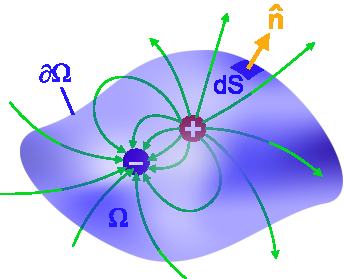
\includegraphics[width=.4\linewidth]{papers/kugel/figures/flux}}
  \caption{
    \label{kugel:fig:eeg}
  }
\end{figure}

To start, we will look at an application that is from the field of medicine:
electroencephalography. The \emph{electroencephalogram} (EEG) is a measurement
of the electrical field on the scalp, which shows the brain's activity, and is
used in many fields of research such as neurology and cognitive psychology.  The
measurement is done by wearing a cap that contains a number of evenly
distributed electrodes, each of which measures the electric potential (voltage)
at their location (figure \ref{kugel:fig:eeg-electrodes}).  To see how this will
relate to the spherical harmonics, we will first quickly recap a bit of physics,
electrodynamics to be precise.

In section \ref{kugel:sec:construction:eigenvalue} we have shown that the
spherical harmonics arise from the surface spherical Laplacian operator, whose
origin we did not consider too much, which is how mathematicians do their work.
On the contrary, physicists usually do the opposite and start by discussing what
is happening in the real world, since variables represent physical quantities.
So, we will quickly remind that the Laplacian operator does the following to an
electric potential $\phi(x, y, z)$:
\begin{equation*}
  \nabla^2 \phi
  = \nabla \cdot \nabla \phi
  = \nabla \cdot \mathbf{E}
  = \rho / \varepsilon,
  \quad \text{or} \quad
  \iiint_\Omega \nabla \cdot \mathbf{E} \, dv
  = \iint_{\partial \Omega} \mathbf{E} \cdot d\mathbf{s}
  = \Phi / \varepsilon.
\end{equation*}
Put into words: on the left we have the differential form, where we recall that
the Laplacian (which is a second derivative) is the divergence of the gradient.
Unpacking the notation we first see that we have the gradient of the potential,
which is just the electric field $\mathbf{E}$, and then the divergence of said
electric field is proportional to the charge density $\rho$. So, the Laplacian
of the electric potential is the charge density! For those that are more
familiar with the integral form of Maxwell's equation, we have also included an
additional step using the divergence theorem, which brings us to the electric
Flux, which by Gauss' law (shown in the iconic\footnote{Every electrical
engineer has seen this picture so many times that is probably burnt in their
eyes.} figure \ref{kugel:fig:eeg-flux}) equals the net electric charge.

Now, an important observation is that if we switch to spherical coordinates, the
physics does not change. So, the spherical Laplacian $\sphlaplacian$ of the
electric potential $\phi(r, \vartheta, \varphi)$ is still the charge density (in
spherical coordinates). And what about the surface spherical Laplacian
$\surflaplacian$? To that case the physics is also indifferent, the only change
is that the units result is a \emph{surface} charge density $\rho_s$. Thus, we
are done with physics and finally arrive at the engineers' perspective: how can
we use this fact to build something that reads the current flows on the surface
of the brain?

The details of how EEG actually works gets very complicated very quickly, but we
will try our best to give an broad overview of the mathematical machinery that
makes it possible to measure brain waves. See, the problem neither the physicist
nor the mathematician considered is that we cannot measure the electric field in
its entirety. As show in figure \ref{kugel:fig:eeg-electrodes} the electrodes
give measurements that are only available at discrete locations, and we are thus
quite a lot of missing data. In other words, we have an interpolation problem.
And (at this point not so surprisingly) we will show that it can be solved using
the spherical harmonics.

To solve this new interpolation problem, we will start with a blatantly
engineering assumption: the human head is a sphere of radius $R$, with the value
of $R$ begin the radius of the average human head. So, we will assume that the
potential distribution on the head can be written as a finite linear combination
of spherical harmonics:
\begin{equation*}
  \phi(\vartheta, \varphi)
    = \sum_{n=0}^N \sum_{m=-n}^n a_{m,n} Y^m_n(\vartheta, \varphi)
\end{equation*}

\subsection{Measuring Gravitational Fields}

\subsection{Quantisation of Angular Momentum}
